\apendice{Documentación técnica de programación}

\section{Introducción}

\section{Estructura de directorios}

\section{Manual del programador}
\subsection{Instalación de \textit{Unity}}

\textit{Unity} \cite{unityweb} en su versión linux puede instalarse de dos maneras: con el archivo .deb y a través de un instalador en forma de script. Ambos archivos se suministran desde la web oficial y se pueden obtener desde el siguiente enlace:

\href{https://forum.unity3d.com/threads/unity-on-linux-release-notes-and-known-issues.350256/}{Web oficial con las versiones de Unity para linux}\footnote{Web oficial Unity: \url{https://forum.unity3d.com/threads/unity-on-linux-release-notes-and-known-issues.350256/}}

La versión utilizada ha sido la 5.3.6f1 que se puede encontrar en:

\href{https://forum.unity3d.com/threads/unity-on-linux-release-notes-and-known-issues.350256/#post-2717623}{Post de la web oficial para la versión 5.3.6f1}\footnote{Unity 5.3.6f1: \url{https://forum.unity3d.com/threads/unity-on-linux-release-notes-and-known-issues.350256/\#post-2717623}}

Y descargar de los siguientes enlaces:

\begin{itemize}
\item Archivo deb: \href{http://download.unity3d.com/download_unity/linux/unity-editor-5.3.6f1+20160720_amd64.deb}{Archivo deb para versión 5.3.6f1}\footnote{Unity 5.3.6f1 archivo deb: \url{http://download.unity3d.com/download_unity/linux/unity-editor-5.3.6f1+20160720_amd64.deb}}

\item Instalador: \href{http://download.unity3d.com/download_unity/linux/unity-editor-installer-5.3.6f1+20160720.sh}{Instalador para versión 5.3.6f1}\footnote{Unity 5.3.6f1 instalador: \url{http://download.unity3d.com/download_unity/linux/unity-editor-installer-5.3.6f1+20160720.sh}}

\item Ambos archivos: \href{http://files.unity3d.com/levi/unity-editor-5.3.6f1+20160720.torrent}{Archivo torrent con ambos archivos}\footnote{Unity 5.3.6f1 ambos archivos: \url{http://files.unity3d.com/levi/unity-editor-5.3.6f1+20160720.torrent}}
\end{itemize}

Para realizar la instalación hemos usado el archivo instalador con los siguientes pasos:
\begin{enumerate}
\item Darle permisos de ejecución con chmod +x al archivo instalador
\item Ejecutar el archivo como superusuario. Crea un directorio donde lo ejecutemos donde se encontraran todos los archivos de Unity.
\end{enumerate}

Para ejecutarlo, hay que ir al nuevo directorio que creó el instalador y ejecutar el ejecutable del editor de Unity que se encuentra dentro de Editor/ 

Para poder usar Monodevelop con la version de Unity, hay que instalar además de la versión que viene con el instalador, el resto de archivos de Monodevelop. Con el comando sudo \textit{apt-get install mono-complete} se instalan desde los repositorios todos los archivos necesarios.

Para comprobar que Unity abrirá el Monodevelop con su versión para Unity, desde el menú \textit{Edit->Preferences}, en la sección \textit{External Tools}, comprobamos que el editor de  los scripts seleccionado es \textit{internal}. Aunque se puede usar cualquier editor para realizar los scripts, es recomendable usar Monodevelop de esta forma porque hay diferencias entre los lenguajes de programación estándar y las versiones de ellos que usa Unity.

También hace falta instalar librerías adicionales de MonoDevelop para poder usar el debugger. Podemos hacerlo desde un terminal con los siguientes comandos:
\begin{itemize}
\item \textit{sudo apt-get install mono-reference-assemblies-2.0}
\item \textit{sudo apt-get install mono-reference-assemblies-3.5}
\item \textit{sudo apt-get install mono-reference-assemblies-4.0}
\end{itemize}

Para usar el \textit{debugger} de MonoDevelop, hay que iniciar el proceso desde el editor de MonoDevelop, usando el botón de ejecución y las opciones de \textit{Debugger} y \textit{Unity Editor} como se ve en la figura \ref{fig:debuggermono}.

\begin{figure}[htpb]
    \centering
    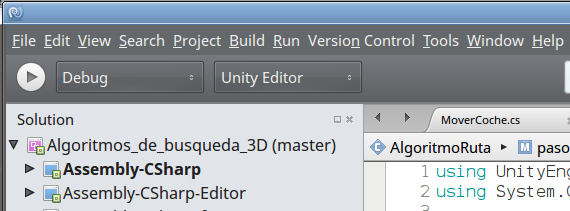
\includegraphics[width=\textwidth,height=4cm,keepaspectratio=true]{d_debuggermono}
    \caption[\textit{Debugger} para \textit{Unity Editor} de MonoDevelop]{\textit{Debugger} para \textit{Unity Editor} de MonoDevelop.}
    \label{fig:debuggermono}
\end{figure}

Entonces nos preguntará a que proceso de \textit{Unity Editor} queremos enlazarlo si no puede hacerlo el mismo. Seleccionamos el proceso de nuestro proyecto (podemos comprobar cual es con un gestor de procesos si no lo sabemos), y MonoDevelop quedará en espera. El proceso de \textit{debug} no comienza hasta que desde el \textit{Unity Editor} iniciemos la ejecución de forma normal, como lo haríamos sin el \textit{debugger}.

\begin{figure}[htpb]
    \centering
    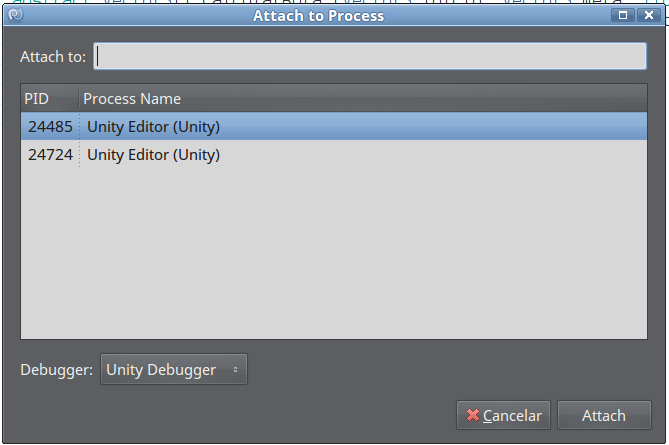
\includegraphics[width=\textwidth,height=6cm,keepaspectratio=true]{d_debuggermono2}
    \caption[Enlace del\textit{Debugger} con \textit{Unity Editor} de MonoDevelop]{Ventana donde se pregunta a que proceso de\textit{Unity Editor} enlazaremos el \textit{Debugger}.}
    \label{fig:debuggermono}
\end{figure}

\subsection{Instalación SmartGit}

Para la organización del repositorio hemos elegido SmartGit, que es un programa disponible de forma gratuita para uso no comercial con versión para linux.

Para su instalación, hay que descargarse el archivo deb de su página web:

\href{https://www.syntevo.com/smartgit/download}{Página de SmartGit}\footnote{SmartGit: \url{https://www.syntevo.com/smartgit/download}}

La versión que hemos utilizado es la 17.0.3 que se puede descargar del siguiente enlace:

\href{https://www.syntevo.com/smartgit/download?file=smartgit/smartgit-17_0_3.deb}{Archivo deb de SmartGit 17.0.3}\footnote{SmartGit 17.0.3: \url{https://www.syntevo.com/smartgit/download?file=smartgit/smartgit-17_0_3.deb}}

El modo de instalación que hemos usado es haciendo doble \textit{click} sobre el archivo deb abriéndolo con el Instalador de software de Ubuntu. También se puede instalar con el comando \textit{dpkg -i nombre-archivo.deb}.

\subsection{Instalación de Texmaker}
Texmaker lo hemos instalado desde los repositorios de Ubuntu usando el gestor con interfaz gráfica Synaptic.

También se puede instalar con el comando \textit{apt-get install textmaker}.

\subsection{Instalación ZenHub}

Para la planificación y control del proyecto hemos usado Zenhub sobre github. Es un complemento de Firefox que añade funciones como las \textit{boards} para manejar el control de las \textit{issues} y las \textit{milestones} del proyecto, y que permite ver los gráficos \textit{burndown} del progreso que se ha realizado.

Para instalarlo, hay que ir a la web oficial
\href{https://www.zenhub.com/}{Web oficial ZenHub}\footnote{Zenhub: \url{https://www.zenhub.com/}}

Pulsando sobre el botón de añadir ZenHub a Github, Firefox nos preguntará si queremos permitir a esa web instalar complementos y debemos darle permiso. A continuación se instalará en Firefox de forma automática y cuando vayamos a nuestro proyecto en github tendremos disponibles la funciones adicionales.

\subsection{Instalación de Remarkable}
Remarkable lo hemos usando el archivo deb descargado de la página oficial. La versión utilizada ha sido la 1.87, que se puede encontrar aquí:

\begin{itemize}
\item \href{https://remarkableapp.github.io/}{Página oficial}\footnote{Remarkable, página oficial: \url{https://remarkableapp.github.io/}}
\item \href{https://remarkableapp.github.io/files/remarkable_1.87_all.deb
}{Archivo deb}\footnote{Remarkable, archivo deb: \url{https://remarkableapp.github.io/files/remarkable_1.87_all.deb}}
\end{itemize}

También se puede instalar con el comando \textit{dpkg -i nombre-archivo.deb}.

\section{Compilación, instalación y ejecución del proyecto}

\section{Pruebas del sistema}
